\section{Operator Spreading in Time-Independent Hamiltonian Systems} \label{sec:opsp}

We will start our discussion of time-independent Hamiltonians with a brief review of unitary time evolution of states and operators. We then define measures of how far an initially local operator has spread over a system. From these we define the butterfly speed $v_B$, which measures how fast operators spread.

Referring back to the introduction, we want a measure of the information spreading in a system. We can define information through commutation, because if two measurements commute, then they do not affect each other. This is equivalent to saying that performing one measurement does not send information to the other measurement. For example, in quantum field theory a correlation function for space-like separated points may be non-zero, but commutation between operators at these points must always vanish, which is to say that information can not travel faster than the speed of light. The velocities we describe will measure how fast the commutators grow.

\subsection{Background: Evolution in Time} \label{sub:evoltime}

All systems considered in this thesis will exist on spin chains, one-dimensional collections of  local quantum degrees of freedom. Initially we consider systems with $q=2$ degrees of freedom at each site, such as a chain of spin-$\half$ particles. Later, we will consider sites with more degrees of freedom. 

Under a time-independent Hamiltonian $H$, states of the system evolve in the Schr\"odinger picture as 
\begin{align}
\ket{\psi(t)} = U(t)\ket{\psi(0)},\quad U(t) = e^{-iHt}. \label{eqn:shro}
\end{align}
Instead of evolving states, it is possible to evolve operators in the Heisenberg picture. In order to preserve the time dependence of expectation values, the operators must evolve as 
\begin{align}
A(t) = U^\dag(t)\,A(0)\,U(t) = e^{iHt}A(0)\,e^{-iHt}.\label{eqn:heis}
\end{align}
There is a slight collision of terminology here. Both $A$ and $U$ are operators, but they play different roles. In this thesis the time evolution operator will always be called a ``unitary operator," or later a ``gate," so that the term ``operator" without qualification always refers to the operator that evolves in time.

One remark worth making about time evolution in different pictures is that operators are not the only the only important Hermitian matrix in the system. The density matrix $\rho$ describes the state of the system, and in pure states is $\rho = \ket{\psi}\bra{\psi}$. Density matrices are more general than kets, though, because they can represent mixed states. In the Schr\"odinger picture $\rho$ evolves the way its construction would imply
\begin{align}
\rho(t) = e^{-iHt}\rho(0)e^{iHt}
\end{align}
while it does not evolve in the Heisenberg picture. This is the opposite of observables, so when discussing the evolution of matrices it is necessary to specify whether they are observables or density matrices.

\subsection{Pauli Strings and Pauli Weight} \label{sub:pauli}

This subsection is based on~\cite{Keyserlingk}. Since it is possible to add Hermitian operators and multiply them by constants, they live in a vector space that can be described using some basis. When discussing operator spreading it is convenient to decompose operators that may act on very high dimensional Hilbert spaces into the Pauli basis. The basis operators are tensor products of Pauli matrices. Eventually we will decompose operators that are initially local, but any operator can be decomposed in this manner.

For single sites with Hilbert spaces of complex dimension $q$, the space of Hermitian operators is $q^2$-dimensional. For $q=2$ the basis operators are $X, Y, Z, I$. In general, there will be two Hermitian operators $X$ and $Z$ that obey $ZX = \exp(2\pi i/q)XZ$ and $Z^q=X^q=I$. Then an arbitrary basis operator will be of the form 
\begin{align}
\sigma^\mu = \phi X^{\mu_1}Z^{\mu_2},
\end{align}
where $\mu_1, \mu_2\in\{0,1,\dots,q-1\}$ and $\phi$ is a phase to preserve Hermiticity. We can extend this description to multiple sites by taking tensor products of $L$ basis operators with subscript $\nu$ representing $L$ $\mu$ indices. Under the matrix norm $||M|| = \text{tr}(M^\dag M)/q^L$, this basis is orthonormal:
\begin{align}
\th{q^L}\text{tr}(\sigma^{\mu\dag}\sigma^\nu) &= \th{q^L}\text{tr}(Z^{\mu_2\dag}
	X^{\mu_1\dag}X^{\nu_1}Z^{\nu_2})\nn
&= \delta_{\mu\nu}.\label{eqn:orthonorm}
\end{align}

A general operator $A = \sum_\nu c_{\nu}(0)\sigma^\nu$ evolves into
\begin{align}
A(t) = U^\dag(t)A\,U(t) = \sum_\nu c_\nu(t)\sigma^\nu.\label{eqn:decomp}
\end{align}
Due to the orthonormality, the coefficients are 
\begin{align}
c_\nu(t) = \th{q^L}\text{tr}(\sigma^{\nu\dag}A(t))
\end{align}
and obey 
\begin{align}
\dt \left(\sum_\nu \abs{c_\nu}^2\right) = 0 \nonumber
\end{align}
due to unitarity. We will consider normalized operators with $\sum_\nu\abs{c_\nu(t)}^2=1$.

With $c_\nu(t)$ in hand, we can define the Pauli weight $W(i,t)$ as how many of the Pauli strings in the decomposition end on site $i$, weighted by their coefficients in Eq.~\ref{eqn:decomp},
\begin{align}
W(i,t) = \sum_\nu\abs{c_\nu(t)}^2\,\delta(\text{end}(\nu)=i).
	\label{eqn:endweight}
\end{align}
The delta function constrains the sum to be only over $\nu$ such that $\sigma^\nu$ has a non-identity at site $i$ and identities at all sites right of $i$. This gives a measure of how far the operator has spread. Reference~\cite{Keyserlingk} refers to this quantity as $\rho$ to emphasize its conservation and hydrodynamic evolution. It is possible to define an analogous quantity with the sum over strings that begin on site $i$ and have identities on all sites left of $i$. In that case the quantity in equation~\ref{eqn:endweight} can be called $W_R(i,t)$ while the weight of sites that start on $i$ is $W_L(i,t)$.

It is helpful to go through an example to explain the Pauli weights. Write
\begin{align}
A = \th{\sqrt{2}} X_0\otimes Y_1\otimes Y_2\otimes I_3 + \th{\sqrt{2}} I_0\otimes I_1\otimes Z_2\otimes Z_3,
	\nonumber
\end{align}
where the subscript designates the site on which each operator acts. This can be shortened to
\begin{align}
A = \th{\sqrt{2}} XYYI + \th{\sqrt{2}} IIZZ\label{eqn:inioper}.
\end{align}
Then the right (ending) Pauli weights are $W_R(i=0) = W_R(i=1) = 0$, $W_R(i=2)= W_R(i=3) =\half$ because one component of the operator ends on site 2 and one ends on site 4. The left (starting) weights are $W_L(i=0) = W(i=2) =\half$, $W_L(i=1) = W_L(i=3)=0$.

This decomposition is particularly useful when the initial operator is local at site $j$. This means that initially all strings in the Pauli decomposition contain non-identity operators only at site $j$ and $W(i,0)=\delta_{ij}$. Then the end weights describe how far the operator has spread throughout the system due to the unitary dynamics, which is an essential feature that allows the systems to thermalize. Figure~\ref{fig:hamspreading} shows the Pauli end weight evolution for an initially local operator in an Ising spin chain with longitudinal field in a strongly chaotic phase~\cite{Jonay17}. The weight moves from site to site and eventually reaches the last site.

\begin{figure}
	\centering
	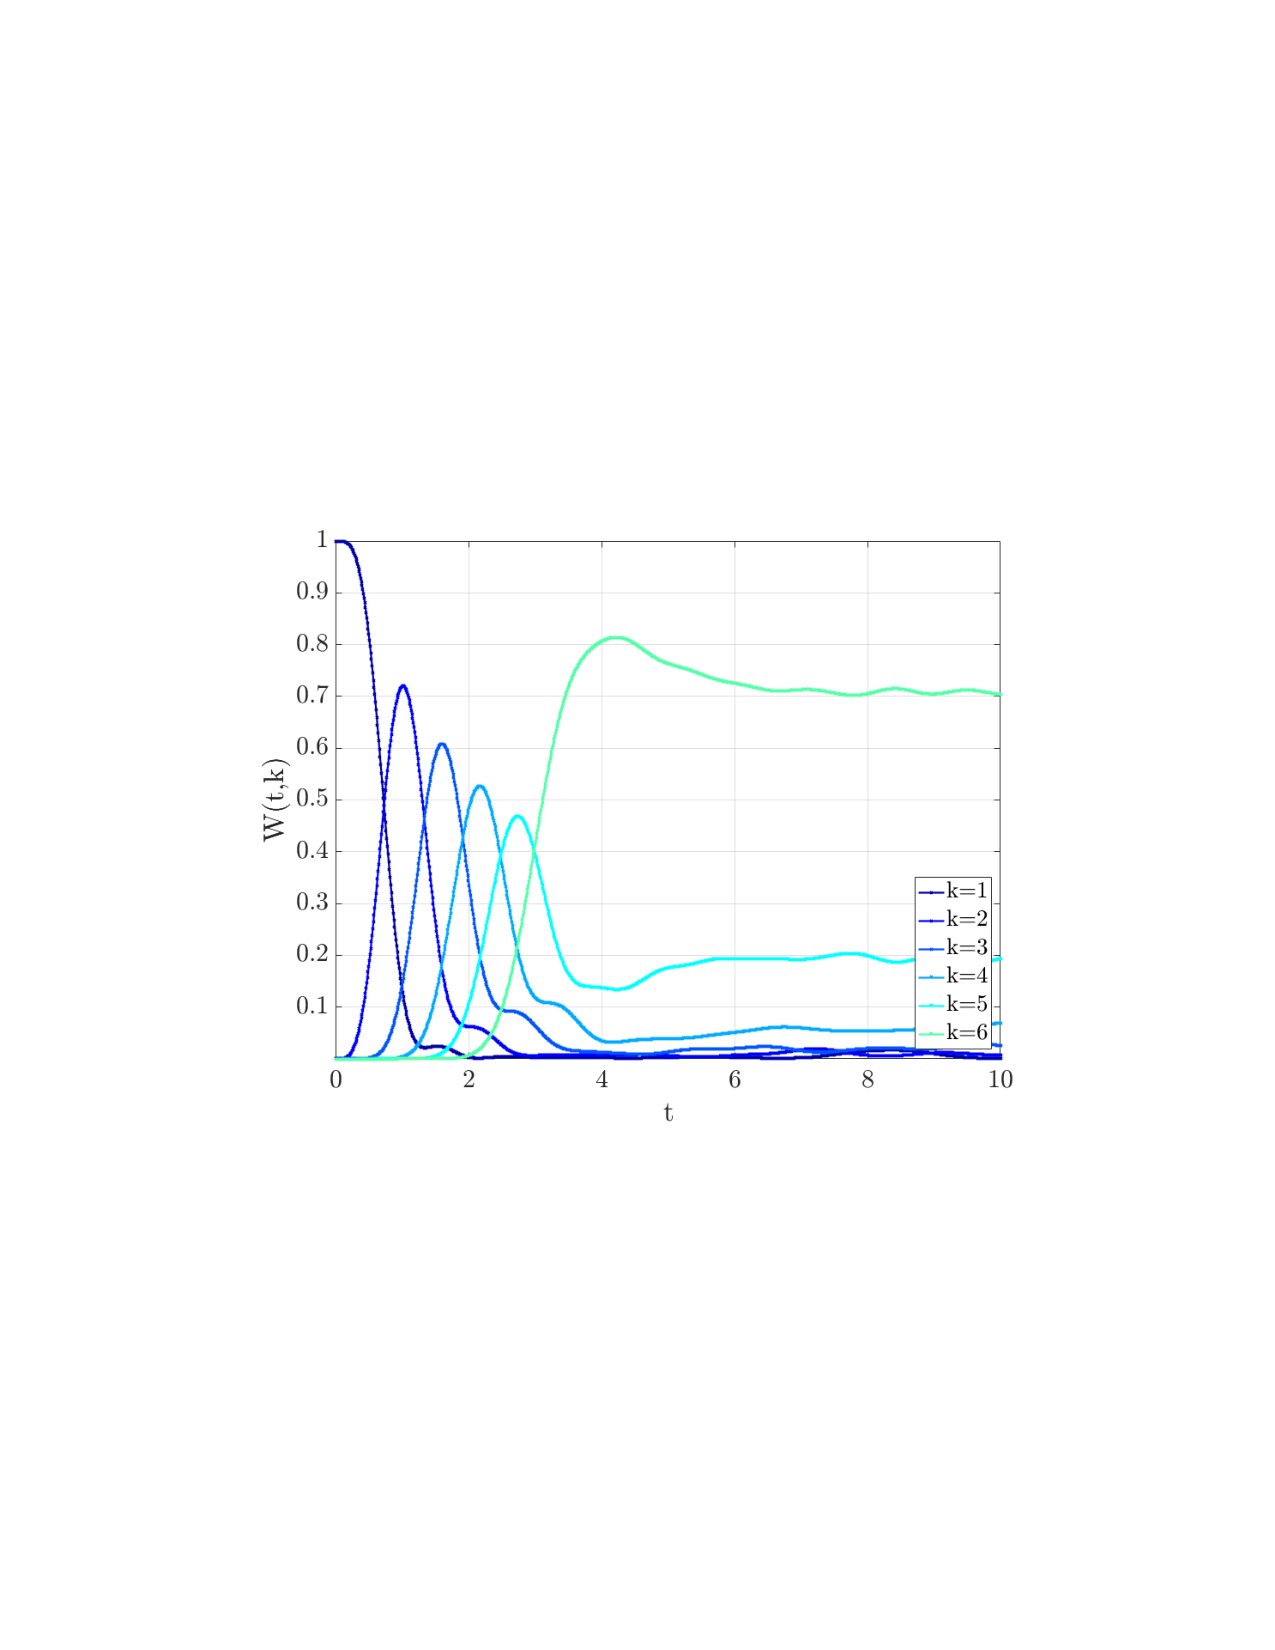
\includegraphics[width=.7\linewidth]{hamspreading}
	\caption{\textbf{Operator spreading as shown by the Pauli weight} in an Ising model with transverse field, from~\cite{Jonay17}. The end weight starts on site 1 and moves sequentially across the system to site 6. Note that the weights at any time sum to 1.}
	\label{fig:hamspreading}
\end{figure}

The Pauli decomposition is related to the Out-of-Time-Ordered Commutator (OTOC). Consider an initial operator, say, $A_0=Z_0=ZII\dots$, where the subscript now indicates the initial location of the operator. This will commute with probe operators that are local at other sites, $B_i$. However, in general the time-evolved $A_0(t)$ will include Pauli strings that have non-identity operators at site $i$. This can be seen through the Baker-Campbell-Hausdorff expansion~\cite{Roberts2016} of the time evolution
\begin{align}
A_0(t) &= e^{iHt}A_0e^{-iHt} \nn
&= \sum_k\frac{(it)^k}{k!}[H,[H,\dots[H,A_0]\dots]],\label{eqn:BCH}
\end{align}
where the dots represent that there are $k$ total commutators taken with $H$.
In general $H$ will contain matrix elements that connect the initially local operator to the non-local strings. Then, $A_0(t)$ can fail to commute with $B_i$, which is still local at $i$ and has not been evolved in time.

The extent to which these two fail to commute can be measured by the OTOC on operators $A_0$ and $B_i$ normalized to $A_0^2=B_i^2=1$,
\begin{align}
C(i,t) = \half\Tr \rho \abs{[A_0(t),B_i]}^2.\nonumber
\end{align}
For a pure state this is equivalent to~\cite{Keyserlingk, Jonay18}
\begin{align}
C(i,t) &= \half\langle\psi|\abs{[A_0(t),B_i]}^2|\psi\rangle\nn
&= 1-\Re\langle\psi|A_0(t)B_iA_0^\dag(t)B_i^\dag|\psi\rangle. \label{eqn:comm}
\end{align}
Some sources define the OTOC using $[A,B]^2$ instead of $|[A,B]|^2$~\cite{Jonay, Roberts2016, Nahum2017}. Others use the acronym to denote the out-of-time-order correlator, $F(i,t) = \ex{A_0(t)B_iA_0^\dag(t)B^\dag_i}$~\cite{Who}, which is related to $C(i,t)$ through Eq.~\ref{eqn:comm}. If $\rho$ is taken to be a thermal state at infinite temperature, the density matrix is proportional to the identity and the OTOC becomes
\begin{align}
C(i,t) = \half\Tr \abs{[A_0(t),B_i]}^2.
\end{align}
This definition can be thought of as independent of the state of the system. We will adopt this as our convention for the OTOC.

To see the relation between this quantity and $W(i,t)$, first consider the case of $q=2$. If the probe is $X_i$ there will be two classes of Pauli strings that commute with it: those with an identity at site $i$ and those with the operator $X$ at site $i$. Then $C(i,t)$ will be the sum of the squares of the $c_\mu(t)$ for which the operator at site $i$ is $Y$ or $Z$. If we average over choice of probe ($X$, $Y$, or $Z$), we arrive at 
\begin{align}
\bar{C}(i,t) = \frac{2}{3}\sum_\nu|c_\nu(t)|^2\,\delta(\text{condition 
	on $\nu$}),\label{eqn:otoc}
\end{align}
where the condition is that the operator at site $i$ is not the identity. This is similar to $W(i,t)$ but measures the weight at $i$. For arbitrary $q$ the prefactor is $\frac{q^2-2}{q^2-1}$. 

If the operator $A_0(t)$ is sufficiently random, all $q^{2L}$ coefficients will have expectation values of the same order, with $|c_\nu|^2 \approx q^{-2L}$. There will be $q^{2L}\frac{q^2-1}{q^2}$ operators that meet the condition, so for these random operators in the large $L$ limit
\begin{align}
\bar{C}(i,t) &= \frac{q^2-2}{q^2-1}q^{2L}\frac{q^2-1}{q^2}\th{q^{2L}}\nn
&= \frac{q^2-2}{q^2}\nonumber.
\end{align}

For $q=2$ there is a particularly easy way to calculate the value in expression~\ref{eqn:otoc}. Since $\Tr(X) = \Tr(Y)=\Tr(Z) = 0$ and $\Tr(I) = 2$, in order to find the non-identity weight at site $i$ start by tracing over the degrees of freedom at that site to obtain $\tilde{A}_0(t) = \half\Tr_iA_0(t)$. Only the strings with the identity at $i$ survive this operation so
\begin{align}
\sum_\nu \abs{c_\nu(t)}^2\delta(\text{condition}) = \frac{3}{2}\bar{C}(i,t) =  \Tr 
	\tilde{A}^\dag_0(t)\tilde{A}_0(t).
\end{align}
We will take this as our definition of the OTOC and relabel it as $C(i,t)$. Using this definition, $\max C(i,t)=1$, and $\ex{C(i,t)}=\frac{3}{4}$ for a random operator with unit norm.

\subsection{Information Velocities} \label{sub:vels}

Since we are studying the spreading of information throughout a system, we want to quantify how fast the information is spreading. In a relativistic system, for example, no information can travel past the speed of light. This is stated precisely by saying that operators at space-like separated points in spacetime must commute. Only within the light cone can two operators have non-zero commutation. Lack of commutation is used as a measure of information transfer because it quantifies how much the two measurements affect each other.

In a spin chain evolving under a Hamiltonian without relativity, there is no requirement that any two operators must commute. This is because of Eqn.~\ref{eqn:BCH}, which can connect distant operators at very small $t$. However, the Lieb-Robinson bound~\cite{Lieb} limits the largest possible commutator of two normalized observables $A_0(t)$ and $B_i$ to
\begin{align}
\abs{\left[A_0(t),B_i\right]}\le K_0 e^{-(\abs{i}-v_{LR}t)/\xi_0},
\end{align}
where $K_0$ and $\xi_0$ are constants and $v_{LR}$ is the Lieb-Robinson velocity, set by the Hamiltonian. Outside $x=v_{LR}$, commutators must be exponentially small, so this is a reasonable ``light cone."

Another velocity that limits the spreading of information in spin chains is the butterfly velocity, the fastest velocity at which perturbations can propagate without decaying exponentially in time. A useful definition of $v_B$ comes from Ref.~\cite{Khemani2018}. In systems large enough so that the site index $i$ can be replaced with a continuous position $x$, the OTOC behaves as~\cite{Khemani2018}
\begin{align}
C(x,t)\sim e^{\lambda(v)t}\quad\text{for}\;\;x=vt.\label{eqn:butterfly}
\end{align}
The condition $x=vt$ tracks the OTOC along rays of constant velocity, as in the lines emanating from the origin in Fig.~\ref{fig:khemani_lambda}.
\begin{figure}
	\centering
	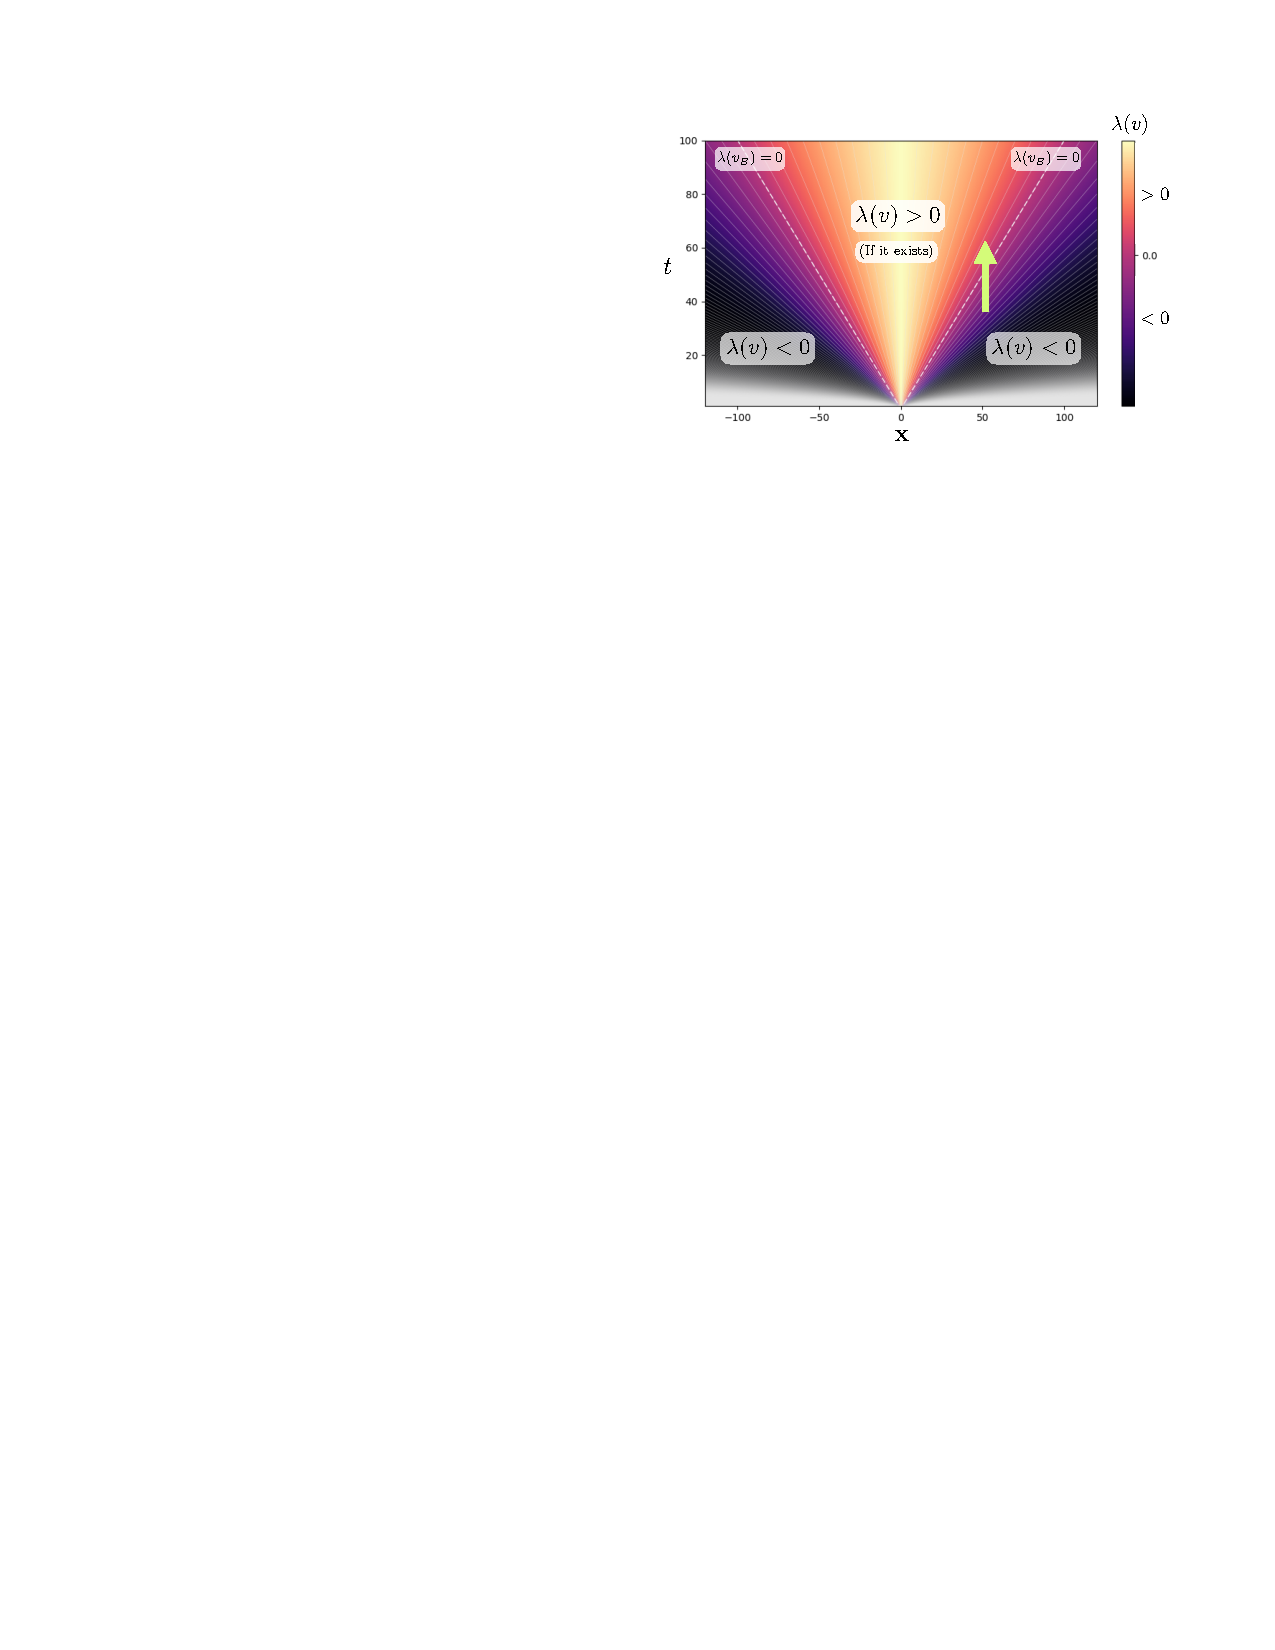
\includegraphics[width=.55\linewidth]{khemani_lambda}
	\caption{\textbf{Velocity dependent Lyapunov exponents} along rays of constant velocity, from~\cite{Khemani2018}. For $v<v_B$, inside the light cone, $\lambda>0$ or is not defined. Outside the light cone $\lambda<0$ and perturbations decay exponentially. The speed $v_B$ is where $\lambda=0$ and perturbations remain of order 1.}
	\label{fig:khemani_lambda}
\end{figure}
The fact that there is a single $v_B$, or possibly one in each direction, is due to the fact that $\lambda(v)$ must be convex, and can only cross 0 once in each direction.

For small velocities in classical chaotic systems, $\lambda$ can be positive, in which case it is the Lyapunov exponent. In analogy, we call the $\lambda(v)$ the velocity-dependent Lyapunov exponent. Typical $\lambda(v)$ in classical and quantum systems can be seen in Fig.~\ref{fig:lyapunov}.
\begin{figure}
	\centering
	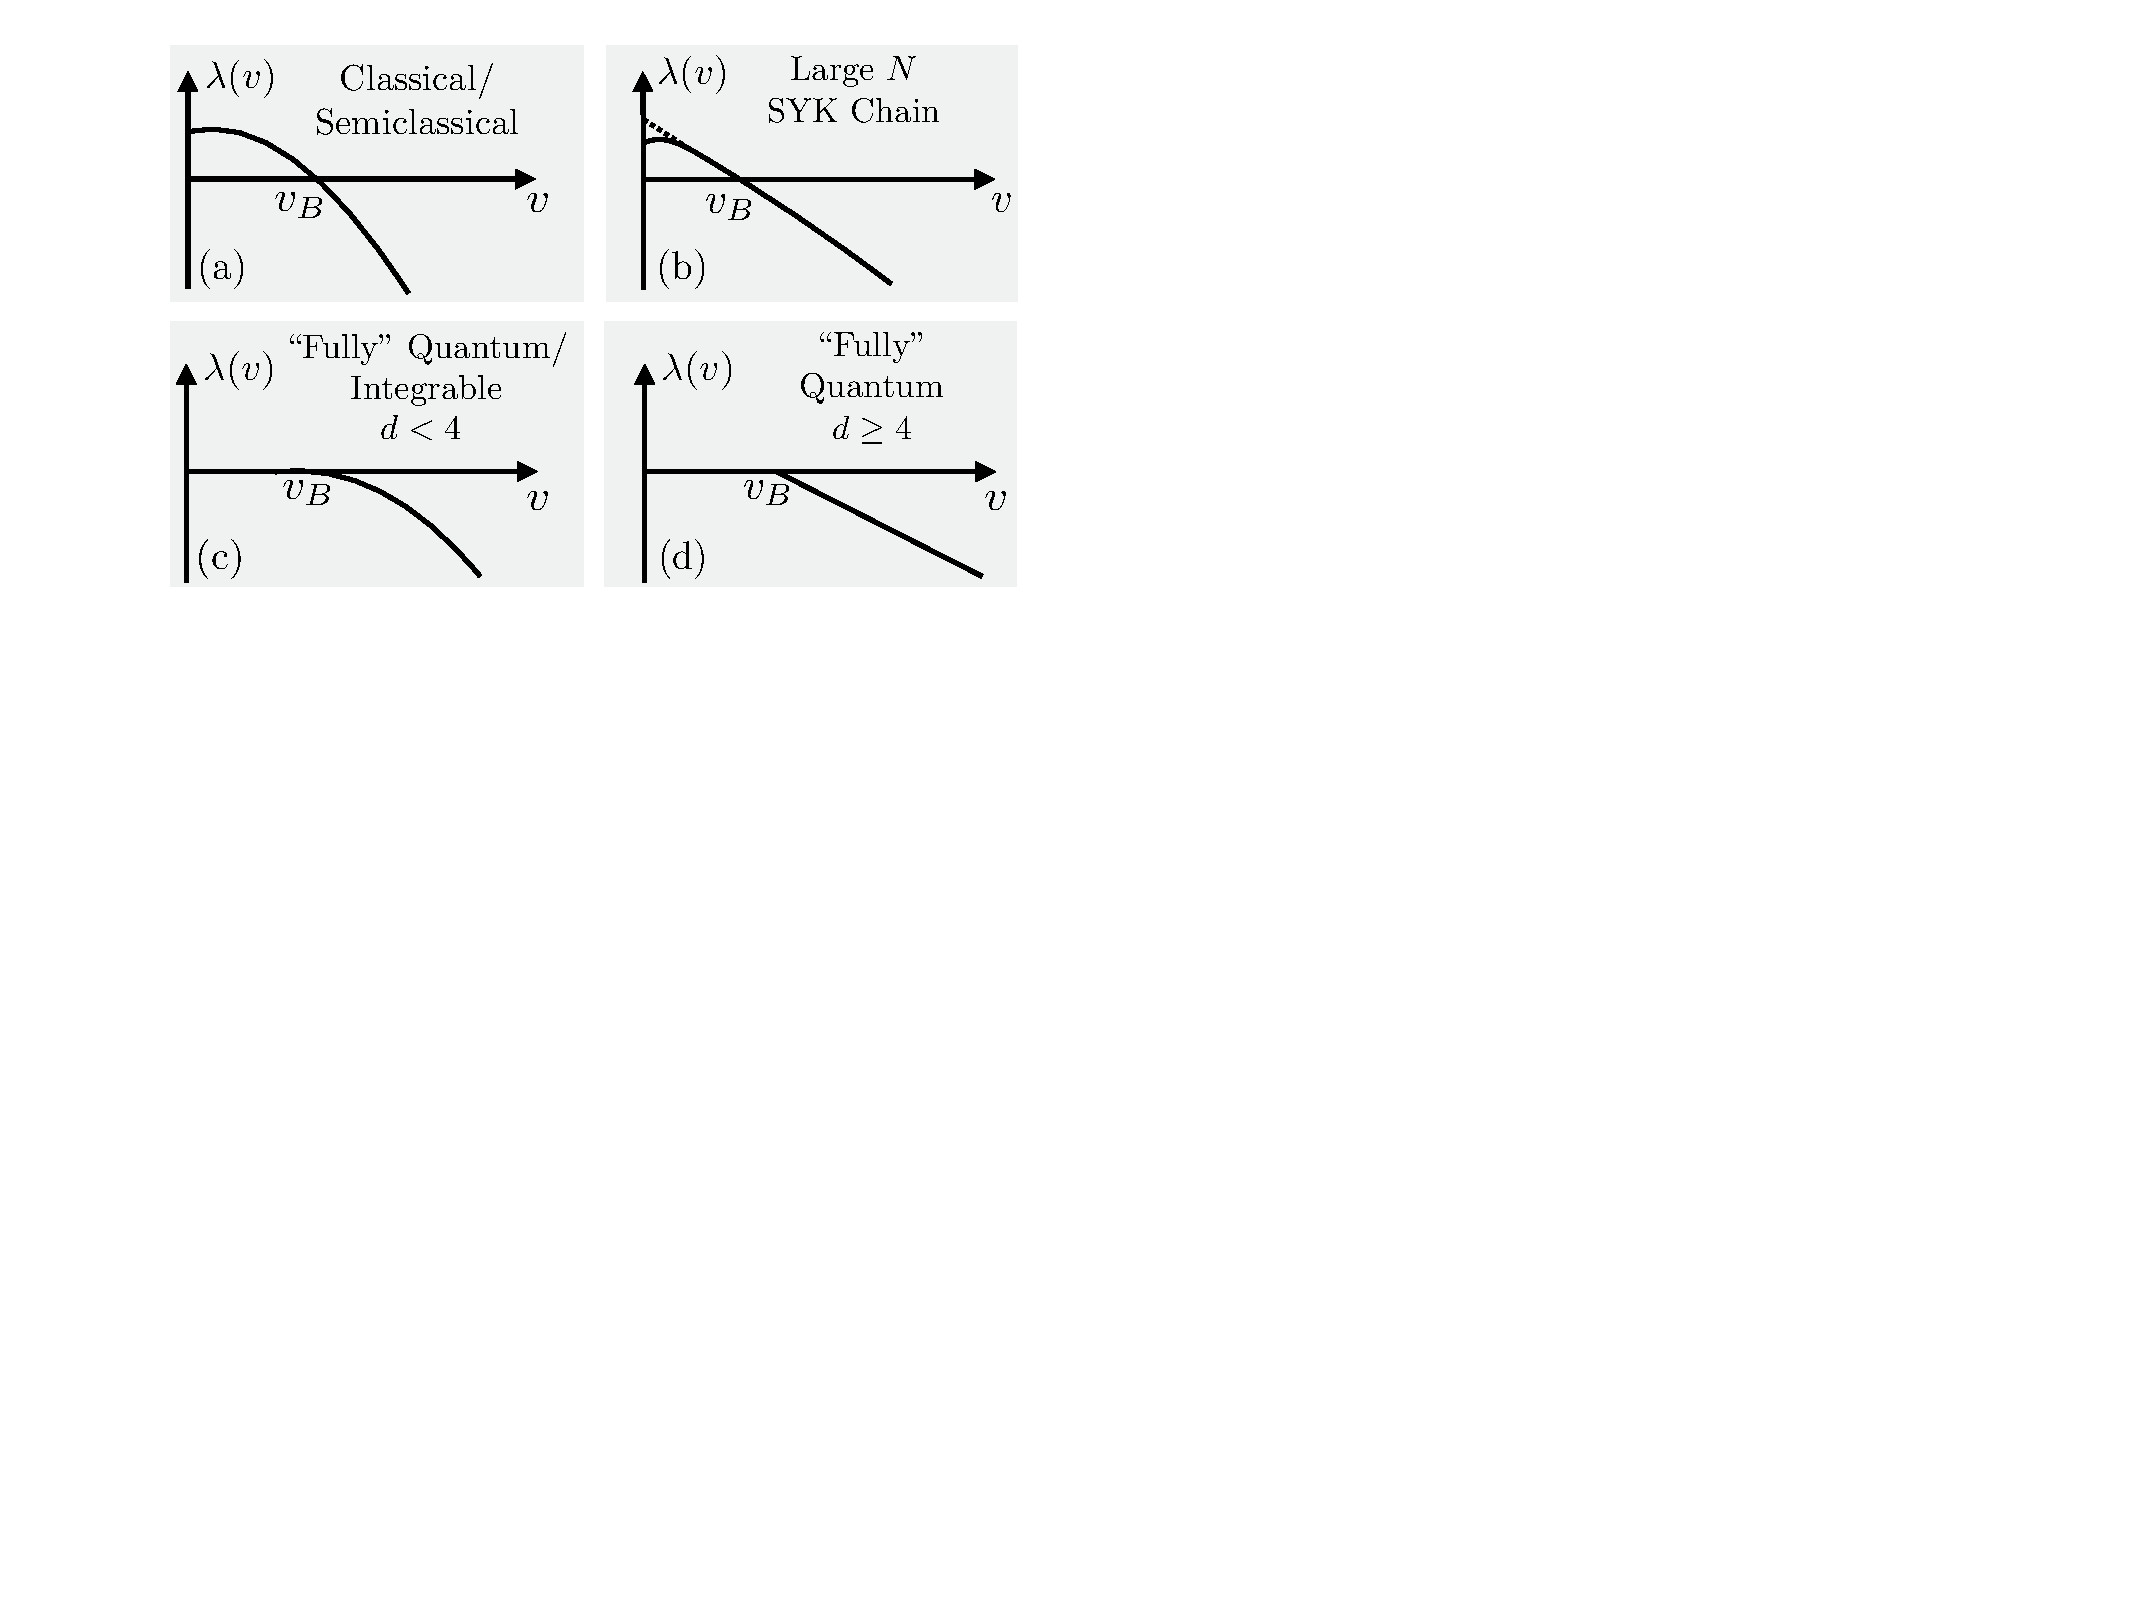
\includegraphics[width=.6\textwidth]{lyapunov}
	\caption{\textbf{Velocity-dependent Lyapunov exponents} in classical and quantum systems. The positive $\lambda$ corresponds to chaos. Figure taken from~\cite{Khemani2018}.}
	\label{fig:lyapunov}
\end{figure}

Note that, for a system with high temperature such that the density operator $\rho\propto\mathbb{I}$, the definitions of $v_{LR}$ and $v_B$ coincide. In general $v_B$ is a ``low-energy analog" of $v_{LR}$~\cite{Roberts2016}. These two speeds can be different, but are not measuring something fundamentally different about the Hamiltonian.

Information dynamics in quantum circuits does have another velocity scale, defined by the entanglement velocity $v_E$. We do not study the entanglement velocity in our Hamiltonian system, but we do in quantum circuits in Sec.~\ref{sec:stairs}. The entanglement velocity is defined in terms of entanglement entropy, which is defined in Sec.~\ref{sec:circuits}. Even without the quantitative definitions, we can still have some understanding of $v_E$.

Two systems $A$ and $B$ are entangled if their joint state $\ket{\Psi}_{AB}$ can not be written as a product state $\ket{\psi_A}_A\ket{\psi_B}_B$. If two parts of a spin chain are initially unentangled and then coupled, they will gradually become entangled. The spins closer to the boundary will become entangled first. The entanglement reaches farther spins at the speed $v_E$.

In general, $v_B/v_E>1$, but the ratio can be made arbitrarily large, as in Ref.~\cite{Nahum2018}. In Sec.~\ref{sec:stairs} we recreate the systems from that reference, but also build systems in which $v_B$ is different in different directions. Before going into more detail about $v_E$, though, we will present systems with time-independent Hamiltonian in which there are two different values of $v_B$.